\documentclass[t]{beamer}
\usetheme{Copenhagen}
\setbeamertemplate{headline}{} % remove toc from headers
\beamertemplatenavigationsymbolsempty

\usepackage{amsmath, array, tikz, bm, pgfplots, tcolorbox, tkz-euclide}
\usetkzobj{all}
\pgfplotsset{compat = 1.16}

\title{Measuring Segments}
\author{}
\date{}

\AtBeginSection[]
{
  \begin{frame}
    \frametitle{Objectives}
    \tableofcontents[currentsection]
  \end{frame}
}

\begin{document}

\begin{frame} 
\maketitle
\end{frame}

\section{Find the distance between two points on a number line.}

\begin{frame}{Measuring Segments}
	To find the distance between two points $A$ and $B$ on a number line, subtract their coordinates and take the absolute value.
	\[ |A - B| \]
\end{frame}

\begin{frame}{Example 1}
	Given the number line below, find each distance.
\begin{center}
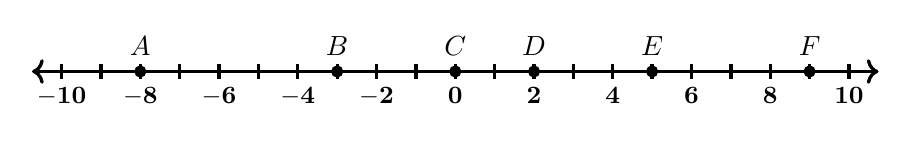
\begin{tikzpicture}[scale = 0.5]
    \foreach \x in {-10, -9, ..., -1, 0, 1, 2, ..., 10}
    \draw[very thick] (\x, 0.2) -- (\x, -0.2);
    \foreach \x in {-10, -8, -6, -4, -2, 0, 2, 4, 6, 8, 10}
    \node at (\x, -0.15) [below] {\small $\mathbf{\x}$};
    \draw[very thick, <->] (-10.75, 0) -- (10.75, 0);
    \draw [fill=black] (-8,0) circle (4pt);
    \node at (-8,0.15) [anchor = south] {$A$};
    \draw [fill=black] (-3,0) circle (4pt);
    \node at (-3,0.15) [anchor = south] {$B$};
    \draw [fill=black] (0,0) circle (4pt);
    \node at (0,0.15) [anchor = south] {$C$};
    \draw [fill=black] (2,0) circle (4pt);
    \node at (2,0.15) [anchor = south] {$D$};
    \draw [fill=black] (5,0) circle (4pt);
    \node at (5,0.15) [anchor = south] {$E$};
    \draw [fill=black] (9,0) circle (4pt);
    \node at (9,0.15) [anchor = south] {$F$};
\end{tikzpicture}
\vspace{10pt}
\end{center}
	(a)	\quad $AC$	\quad	\pause    8   \newline\\  \pause
    (b) \quad $BE$  \quad   \pause    8     \newline\\  \pause
    (c) \quad $CF$  \quad   \pause    9
\end{frame}

\section{Work with congruent segments}

\begin{frame}{Congruent Segments}
In the previous example, both $\overline{AC}$ and $\overline{BE}$ had lengths of 8. \newline\\  \pause

We would say that $\overline{AB}$ is congruent to $\overline{BE}$.  \newline\\  \pause

\begin{tcolorbox}[colframe=green!20!black, colback = green!30!white,title=\textbf{Congruent Segments}]
Two segments are \textbf{congruent} if they have the same length.
\end{tcolorbox}
\vspace{8pt} \pause

The symbol for congruent is $\cong$ \quad   $\overline{AB} \cong \overline{BE}$ \newline\\  \pause

We mark congruent segments using tick marks.
\end{frame}

\begin{frame}{Example 2}
(a) \quad Find the value of $x$ if $\overline{AB} \cong \overline{CD}$.  
\begin{center}
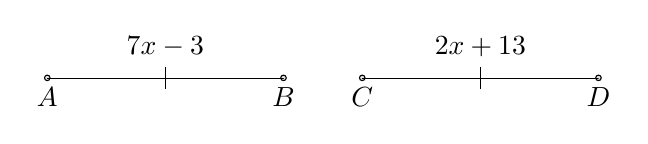
\begin{tikzpicture}
\tkzDefPoints{0/0/A, 3/0/B, 4/0/C, 7/0/D}
\tkzDrawPoints(A,B,C,D)
\tkzDrawSegments(A,B C,D)
\tkzLabelPoints[below](A,B,C,D)
\tkzMarkSegments[mark=|](A,B C,D)
\tkzLabelSegment[above,yshift=4pt](A,B){$7x-3$}
\tkzLabelSegment[above,yshift=4pt](C,D){$2x+13$}
\end{tikzpicture}
\end{center}
\begin{align*}
    \onslide<2->{7x-3 &= 2x+12} \\
    \onslide<3->{5x -3 &= 12} \\
    \onslide<4->{5x &= 15}  \\
    \onslide<5->{x &= 3}
\end{align*}
\onslide<6->{Check:}
\begin{align*}
\onslide<7->{7(3)-3 &= 2(3)+12?}    \\
\onslide<8->{18 &= 18}
\end{align*}
\end{frame}

\begin{frame}{Example 2}
(b) \quad Find the values of $x$ and $y$
\begin{center}
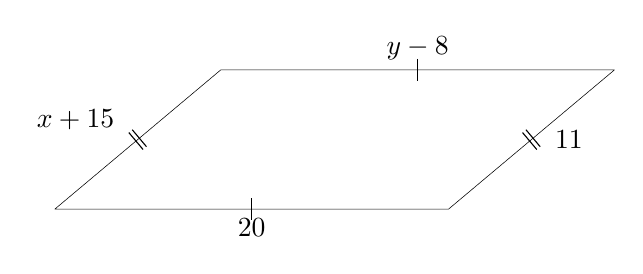
\begin{tikzpicture}
\tkzDefPoints{0/0/A, 5/0/B}
\tkzDefShiftPoint[A](40:2.75){C}
\tkzDefShiftPoint[B](40:2.75){D}
\tkzDrawPolygon(A,B,D,C)
\tkzMarkSegments[mark=|](A,B C,D)
\tkzMarkSegments[mark=||](A,C B,D)
\tkzLabelSegment[above left,xshift=-5pt](A,C){$x+15$}
\tkzLabelSegment[right,xshift=5pt](B,D){11}
\tkzLabelSegment[above](C,D){$y-8$}
\tkzLabelSegment[below](A,B){20}
\end{tikzpicture}
\end{center}
\begin{align*}
\onslide<2->{x+15&=11 & y-8&=20} \\
\onslide<3->{x&=-4 & y&=28}
\end{align*}
\end{frame}

\section{Use the Segment Addition Postulate}

\begin{frame}{Segment Addition Postulate}
If 3 points $A$, $B$, and $C$ are collinear and $B$ is between $A$ and $C$, then \[AB + BC = AC\]    \vspace{10pt}
\begin{center}
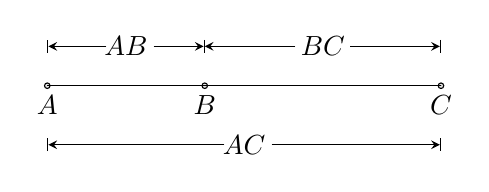
\begin{tikzpicture}
\tkzDefPoints{0/0/A, 2/0/B, 5/0/C}
\tkzDrawPoints(A,B,C)
\tkzLabelPoints[below](A,B,C)
\tkzDrawSegment(A,C)
\node at (1,0.5) {$AB$};
\node at (3.5,0.5) {$BC$};
\node at (2.5,-0.75) {$AC$};
\draw [->|, >=stealth](0.75,0.5) -- (0,0.5);
\draw [->|, >=stealth](1.35,0.5) -- (2,0.5);
\draw [->, >=stealth](3.15,0.5) -- (2,0.5);
\draw [->|, >=stealth](3.85,0.5) -- (5,0.5);
\draw [->|, >=stealth](2.25,-0.75) -- (0,-0.75);
\draw [->|, >=stealth](2.85,-0.75) -- (5,-0.75);
\end{tikzpicture}
\end{center}
\end{frame}

\begin{frame}{Example 3}
(a) \quad   If $EG=59$, what are $EF$ and $FG$? 
\begin{center}
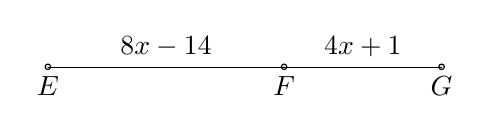
\begin{tikzpicture}
    \tkzDefPoints{0/0/E, 3/0/F, 5/0/G}
    \tkzDrawPoints(E,F,G)
    \tkzLabelPoints[below](E,F,G)
    \tkzDrawSegment(E,G)
    \tkzLabelSegment[above](E,F){$8x-14$}
    \tkzLabelSegment[above](F,G){$4x+1$}
\end{tikzpicture}
\end{center}
\begin{align*}
\onslide<2->{EF + FG &= EG} \\
\onslide<3->{8x-14 + 4x+1 &= 59} \\
\onslide<4->{12x - 13 &= 59} \\
\onslide<5->{12x &= 72} \\
\onslide<6->{x &= 6}
\end{align*}
\begin{align*}
\onslide<7->{EF &= 8(6)-14 & FG &= 4(6)+1} \\
\onslide<8->{EF &= 34 & FG &= 25}
\end{align*}
\end{frame}

\begin{frame}{Example 3}
(b) \quad If $JL=120$, what are $JK$ and $KL$?  
\begin{center}
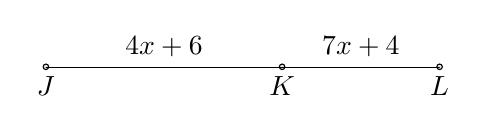
\begin{tikzpicture}
    \tkzDefPoints{0/0/J, 3/0/K, 5/0/L}
    \tkzDrawPoints(J,K,L)
    \tkzLabelPoints[below](J,K,L)
    \tkzDrawSegment(J,L)
    \tkzLabelSegment[above](J,K){$4x+6$}
    \tkzLabelSegment[above](K,L){$7x+4$}
\end{tikzpicture}
\end{center}
\begin{align*}
\onslide<2->{JK + KL &= JL} \\
\onslide<3->{4x+6 + 7x+4 &= 120} \\
\onslide<4->{11x +10 &= 120} \\
\onslide<5->{11x &= 110} \\
\onslide<6->{x &= 10}
\end{align*}
\begin{align*}
\onslide<7->{JK &= 4(10)+6 & KL &= 7(10)+4} \\
\onslide<8->{JK &= 46 & KL &= 74}
\end{align*}
\end{frame}

\section{Use the midpoint of a segment.}

\begin{frame}{Midpoint}
\begin{tcolorbox}[colframe=green!20!black, colback = green!30!white,title=\textbf{Midpoint}]
A \textbf{midpoint} divides a segment into 2 congruent segments.
\end{tcolorbox}
\vspace{8pt} \pause

In the picture below, $B$ is the midpoint of $\overline{AC}$.
\newline\\
\begin{center}
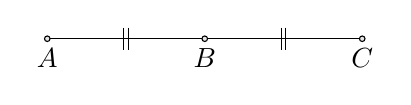
\begin{tikzpicture}
    \tkzDefPoints{0/0/A, 2/0/B, 4/0/C}
    \tkzDrawSegment(A,C)
    \tkzDrawPoints(A,B,C)
    \tkzLabelPoints[below](A,B,C)
    \tkzMarkSegments[mark = ||](A,B B,C)
\end{tikzpicture}
\end{center}
\end{frame}

\begin{frame}{Example 4}
(a) \quad   $Q$ is the midpoint of $PR$. What are $PQ$, $QR$, and $PR$?
\begin{center}
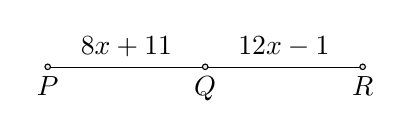
\begin{tikzpicture}
    \tkzDefPoints{0/0/P, 2/0/Q, 4/0/R}
    \tkzDrawSegment(P,R)
    \tkzDrawPoints(P,Q,R)
    \tkzLabelPoints[below](P,Q,R)
    \tkzLabelSegment[above](P,Q){$8x+11$}
    \tkzLabelSegment[above](R,Q){$12x-1$}
\end{tikzpicture}
\end{center}
\begin{align*}
\onslide<2->{8x+11 &= 12x-1} \\
\onslide<3->{11 &= 4x-1} \\
\onslide<4->{12 &= 4x} \\
\onslide<5->{x &= 3}
\end{align*}
\begin{align*}
\onslide<6->{PQ &= 8(3)+11 & QR &= 12(3)-1 & PR &= PQ + QR} \\
\onslide<7->{PQ &= 35 & QR &= 35 & PR &= 35 + 35 = 70}
\end{align*}
\end{frame}

\begin{frame}{Example 4}
(b) \quad   $U$ is the midpoint of $TV$. What are $TU$, $UV$, and $TV$?
\begin{center}
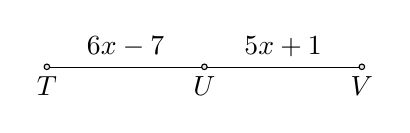
\begin{tikzpicture}
    \tkzDefPoints{0/0/T, 2/0/U, 4/0/V}
    \tkzDrawSegment(T,V)
    \tkzDrawPoints(T,U,V)
    \tkzLabelPoints[below](T,U,V)
    \tkzLabelSegment[above](T,U){$6x-7$}
    \tkzLabelSegment[above](U,V){$5x+1$}
\end{tikzpicture}
\end{center}
\begin{align*}
\onslide<2->{6x-7 &= 5x+1} \\
\onslide<3->{x-7 &= 1} \\
\onslide<4->{x &= 8}
\end{align*}
\begin{align*}
\onslide<5->{TU &= 6(8)-7 & UV &= 5(8)+1 & TV &= TU+UV} \\
\onslide<6->{TU &= 41 & UV &= 41 & PR &= 41 + 41 = 82}
\end{align*}
\end{frame}

\end{document}
